\chapter{Related Work}

In prezent, exista mai multi algoritmi genetici ce sunt devoltati pentru a perfectiona o actiune fizica sau pentru a optimiza probleme prin selectie naturala. 
\section{Locomotie prin algoritmi evolutivi}

\subsection{Cell Evolution}
O incercare de a simula evolutia locomotiei de la un nivel celular apare in articolul \textbf{Fine grained artificial development for body-controller coevolution of soft-bodiedanimats} \footnote{\url{https://www.mitpressjournals.org/doi/pdf/10.1162/978-0-262-32621-6-ch040}} \footnote{\url{https://www.youtube.com/watch?v=CXTZHHQ7ZiQ}}. 

Procesul evolutionar incepe de la o singura celula ce sufera divizie celulara. O celula este reprezentata de un disc ce sufera coliziuni elastice simulate prin arcuri cu alte celule. O celula are o pozitie, viteza, si o orientare ce reprezinta directia diviziunii celulare. O celula se poate "contracta" iar compartamenul acesteia este controlat de o retea neuronala si poate fi afectata de celulele din jur.

Pentru procesul de evolutie a fost folosit \textbf{NEAT}\footnote{\url{http://nn.cs.utexas.edu/downloads/papers/stanley.ec02.pdf}}, \textit{neuroevolution of augmenting topologies  Stanley  and  Miikkulainen,  2002}. Populatia aleasa a fost $\lambda = 300$ cu genomi de lungimi arbitrare si 2000 de generatii.

\begin{center}
    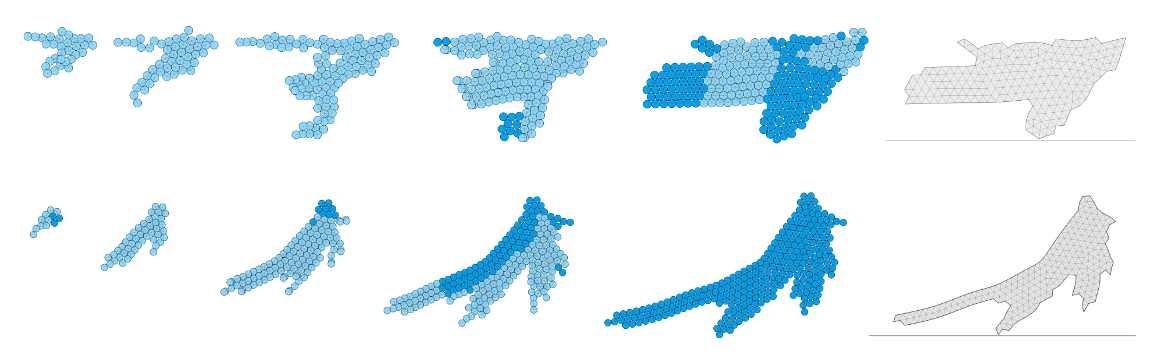
\includegraphics[width=1\textwidth]{cellular_evolution.png}\linebreak
    \textit{source: \url{https://www.mitpressjournals.org/doi/pdf/10.1162/978-0-262-32621-6-ch040}}\linebreak
    \textit{video example: \url{https://www.youtube.com/watch?v=Q6XXohgPP4A&feature=youtu.be}}
\end{center}

Evolutia unui embrion rezultat. Fiecare celula luminoasa reprezinta o celula ce este pregatita de divzie celulara.

\subsection{Muskoscheletal Evolution}
Articolul \textbf{Flexible Muscle-Based Locomotion for Bipedal Creatures}\footnote{\url{https://www.cs.ubc.ca/~van/papers/2013-TOG-MuscleBasedBipeds/2013-TOG-MuscleBasedBipeds.pdf}} ce a simulat locomotia prezinta un algoritm evolutiv ce foloseste CMA-ES \footnote{\url{https://en.wikipedia.org/wiki/CMA-ES}} (\textit{covariance matrix adaptation evolution strategy}) cu o populatie $\lambda = 20$ si step-size $\sigma = 1$. Modul in care au optimizat problema a fost de a minimiza eroarea $E(K)$:\begin{center} $E(K) = E_{speed} + E_{headori}+ E_{headvel}+ E_{slide}+ E_{effort}$ \end{center}

Acestia reusesc sa optimizeze un set de muschi si incheieturi 3D pentru a obtine indivizi finali, care pot ajunge la o viteza dorita, fac fata unui teren inegal si a evenimentelor externe.
\subsection{Joint Evolution}
Un alt algoritm genetic, numit \textbf{Genetic Walkers} \footnote{\url{https://rednuht.org/genetic_walkers/}} incearca sa simuleze o miscare in 2D. Spre deosebire de abordarea anterioara acest algoritm optimizeaza distanta dintre \textit{head} fata de \textit{feet}, distanta pe care fiecare individ reuseste sa o parcurga. De asemenea fiecare individ primeste 100 de puncte in fitness pentru fiecare pas corect realizat. Spre deosebire de primul articol, selectia se realizeaza prin o functie $f$, $f(k) = \frac{1}{k+2}$, unde $k$ este indexul unui cromozom, ordonati in ordinea fitnessului. Primii doi cromozomi alesi vor realiza un copil in generatia urmatoare. Optimizarea se face asupra unghiului unui joint si a duratei de timp.

\subsection{Concluzii}
Ambii algoritmi lucreaza cu un corp 3D fixat de la inceput, dar evolueaza miscarea in moduri diferite, unul lucureazaza low-level, cu un schelet muscular iar altul strict cu rotatia unui joint. Algoritmul low level produce rezultate \footnote{\url{https://www.youtube.com/watch?v=pgaEE27nsQw}} mult mai fidele in timp ce al doilea algoritm reuseste sa faca ~3 pasi dupa 500 de generatii.

\pagebreak
\section{Algoritmi evolutivi in cercetare}

\subsection{Evolved Antenna}

In radio comunicatii, o \textbf{Antena Evoluata} \footnote{\url{https://en.wikipedia.org/wiki/Evolved_antenna}} repreza o antena proiectata complet sau partial de un algoritm genetic. 

Pentru a gasi solutii pentru probleme noi, cum ar fi detectarea anumitor radiatii, au fost incercati algoritmii genetici, iar in 2006, in cadrul misiunii \textit{Space Technology 5} \footnote{\url{https://ti.arc.nasa.gov/m/pub-archive/1244h/1244\%20(Hornby).pdf}}, a fost dezvoltata prima antena folosita in spatiu. Urmatoarele doua antene au fost proiectate de catre un algoritm genetic:
\begin{center}
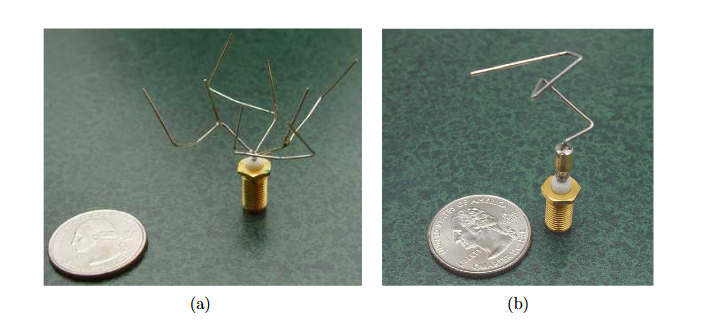
\includegraphics[width=1\textwidth]{evolved_antenna.png}
source: \textit{https://ti.arc.nasa.gov/m/pub-archive/1244h/1244\%20(Hornby).pdf}
\end{center}